\documentclass[a4paper,14pt]{article}

\usepackage[T2A]{fontenc}
\usepackage[utf8]{inputenc}
\usepackage[russian]{babel}
\usepackage{graphicx}
\usepackage[left=1cm,right=1cm,bottom=1cm,top=2cm]{geometry}
\usepackage{hyperref}
\title{Приложение к ленте времени}
\author{Егор Федоров, P3115}
\date{Октябрь 2022 г.}

\usepackage{fancyhdr}
\fancyhead[L]{Федоров Егор, P3115}
\fancyhead[R]{Приложение к ленте времени}
\fancyfoot{}

\begin{document}
\pagestyle{fancy}
\section*{Древняя Русь}
\textbf{Жилье восточных славян} --- (рис.~\ref{fig:slavs}) картина С.В. Иванова

\textbf{Великий Новгород (859 г.)} --- (рис.~\ref{fig:novrogod}) картина А.М. Васнецова (1901 г.)

\textbf{Призвание варягов (862 г.)} --- (рис.~\ref{fig:summon}) картина Виктора Михайловича Васнецова (1909 г.)

\textbf{Тризна дружинников Святослава после боя под Доростолом в 971 году} (рис.~\ref{fig:trizna}) --- картина Генриха Семирадского, (1881-1882 гг.)

\textbf{Крещение Руси (988 г.)} --- (рис.~\ref{fig:chresh}) фреска Виктора Михайловича Васнецова в киевском Владимирском монастыре (1895-1896 гг.)

\textbf{Свержение идолов в Киеве (988 г.)} (рис.~\ref{fig:sverzh}) --- картина А.И. Беглова, 1990 г.

\textbf{Битва при Немиге (1067 г.)} --- (рис.~\ref{fig:nemiga}) миниатюра из Радзивилловской летописи

\textbf{Русские князья заключают мир в Уветичах (1100 г.)} (рис.~\ref{fig:uvetichi}) --- картина С.В. Иванова, 

\textbf{Битва при Салнице (1111 г.)} --- (рис.~\ref{fig:salnitsa}) миниатюра из Радзивилловской летописи

\textbf{Битва на Калке (1223 г.)} --- (рис.~\ref{fig:kalka}) картина современного художника Зябкина Дмитрия, 2007 г.

\section*{Византийская Империя}
\textbf{Бюст Феодосия II (401 - 450)} --- (рис.~\ref{fig:theodosius}) мрамор, 5 век


\textbf{Мозаика Юстиниана I} --- (рис.~\ref{fig:justinianus}) базилика Сан-Витале в Равенне, 527 -- 548 год

\textbf{Битва при Ярмуке (636 г.)} --- (рис.~\ref{fig:yarmuka}) анонимный католический иллюстратор (между 1310 и 1325 годом)

\textbf{Святой Мокий Амфипольский и ангел, убивающий иконоборцев. 1066 год} (рис.~\ref{fig:ikoni})  - миниатюра из Псалтыри Феодора Кесарийского

\textbf{Дочери императрицы Феодоры учатся почитать иконы у бабушки Феоктисты} (рис.~\ref{fig:feodora})  - миниатюра из мадридского кодекса «Хроники» Иоанна Скилицы. XII–XIII века 

\textbf{Христос, благословляющий Константина Багрянородного} (рис.~\ref{fig:christ})  -  резьба по слоновой кости, ок. 945 г.

\textbf{Ангелы возлагают на Василия II императорскую корону} (рис.~\ref{fig:angels}) - миниатюра из Псалтыри Василия, Библиотека Марчиана. XI век
\textbf{Битва при Дорилее (1097 г.)} (рис.~\ref{fig:dorilee}) --- миниатюра Жака Коломба из книги Себастьена Мамро <<Походы французов в Утремер>>

\textbf{Участники Второго крестового похода (1145—1149) прибывают в Константинополь} (рис.~\ref{fig:crusaders_2}) - Миниатюра из <<Больших французских хроник>> 

\textbf{Взятие Константинополя крестоносцами (1204 г.)} (рис.~\ref{fig:crusaders_3}) - картина Делакруа, 1840 г.

\section*{Западная Европа}
\textbf{Крещение Хлодвига} (рис.~\ref{fig:clovis}) --- миниатюра из <<Больших хроник Франции>>, 25 декабря 496 г.

\textbf{Гунтрамн и Хильдеберт} (рис.~\ref{fig:gunt}) --- миниатюра из <<Больших хроник Франции>>, 561 -- 592 гг.

\textbf{Битва при Пуатье (732 г.)} (рис.~\ref{fig:poitiers}) --- картина Карла Штейбена, дата написания: 1834 --- 1837 гг.


\textbf{Людовик I Благочестивый, император Запада} (рис.~\ref{fig:louis}) --- картина Жана-Жозефа Дасси, дата написания: 1837 г.

\textbf{Свадьба Гуго и Мароции} (рис.~\ref{fig:gugo}) ---  гравюра XIX века из книги Ф. Бертолини

\textbf{Генрих I. Король Франции} (рис.~\ref{fig:henry}) --- картина М.-Ж. Блонделя, дата написания: 1837 г.

\textbf{Коронация Людовика VI} (рис.~\ref{fig:corona}) --- миниатюра из <<Больших французских хроник>> 

\textbf{Свадьба Алиеноры Аквитанской и Людовика VII} (рис.~\ref{fig:henry}) --- картина М.-Ж. Блонделя, дата написания: 1837 г.

\textbf{Осада Тира (1187)} (рис.~\ref{fig:tyr}) --- миниатюра Жана Коломба из книги Себастьена Мамро <<Походы французов в Утремер>> (1474)

\textbf{Людовик IX с войсками в Крестовом походе} (рис.~\ref{fig:crusaders})  --- миниатюра из <<Жития и чудес Св. Людовика>> Гийома де Сен-Патю. 1330-1340 гг.

\begin{figure}[ht]
    \centering
    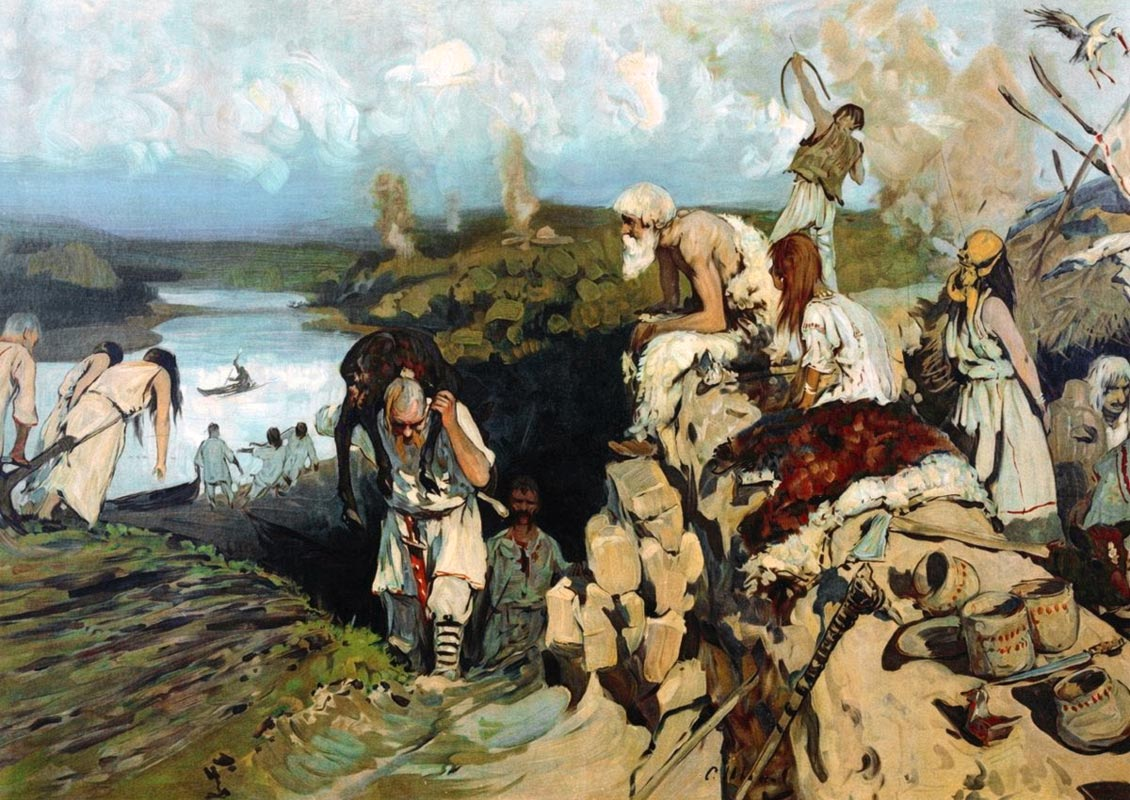
\includegraphics[width=0.45\textwidth]{img/rus/Living_of_East_Slavs_by_Ivanov.jpg}
    \caption{Жилье восточных славян}
    \label{fig:slavs}
\end{figure}

\begin{figure}[ht]
    \centering
    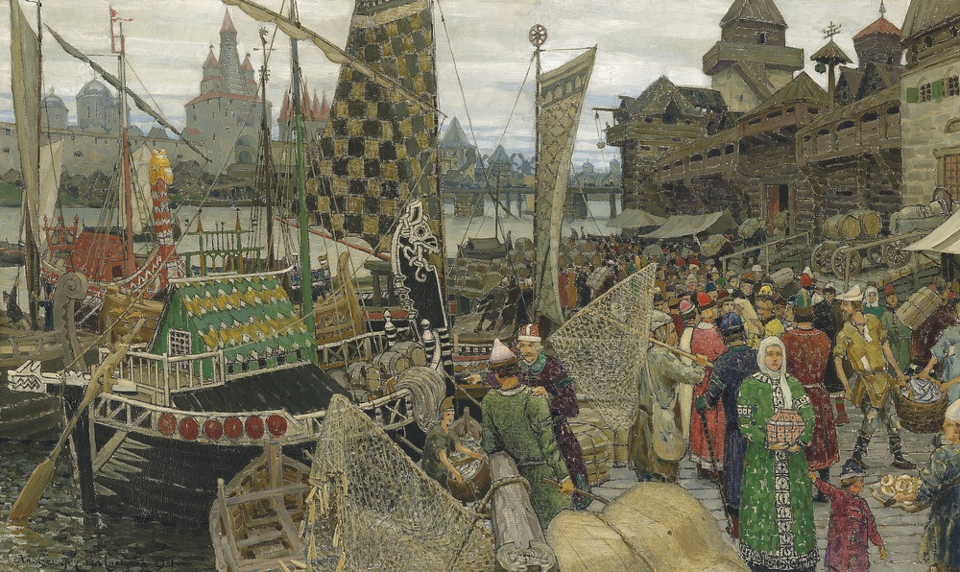
\includegraphics[width=0.45\textwidth]{img/rus/novgorod.png}
    \caption{Великий Новгород}
    \label{fig:novrogod}
\end{figure}

\begin{figure}[ht]
    \centering
    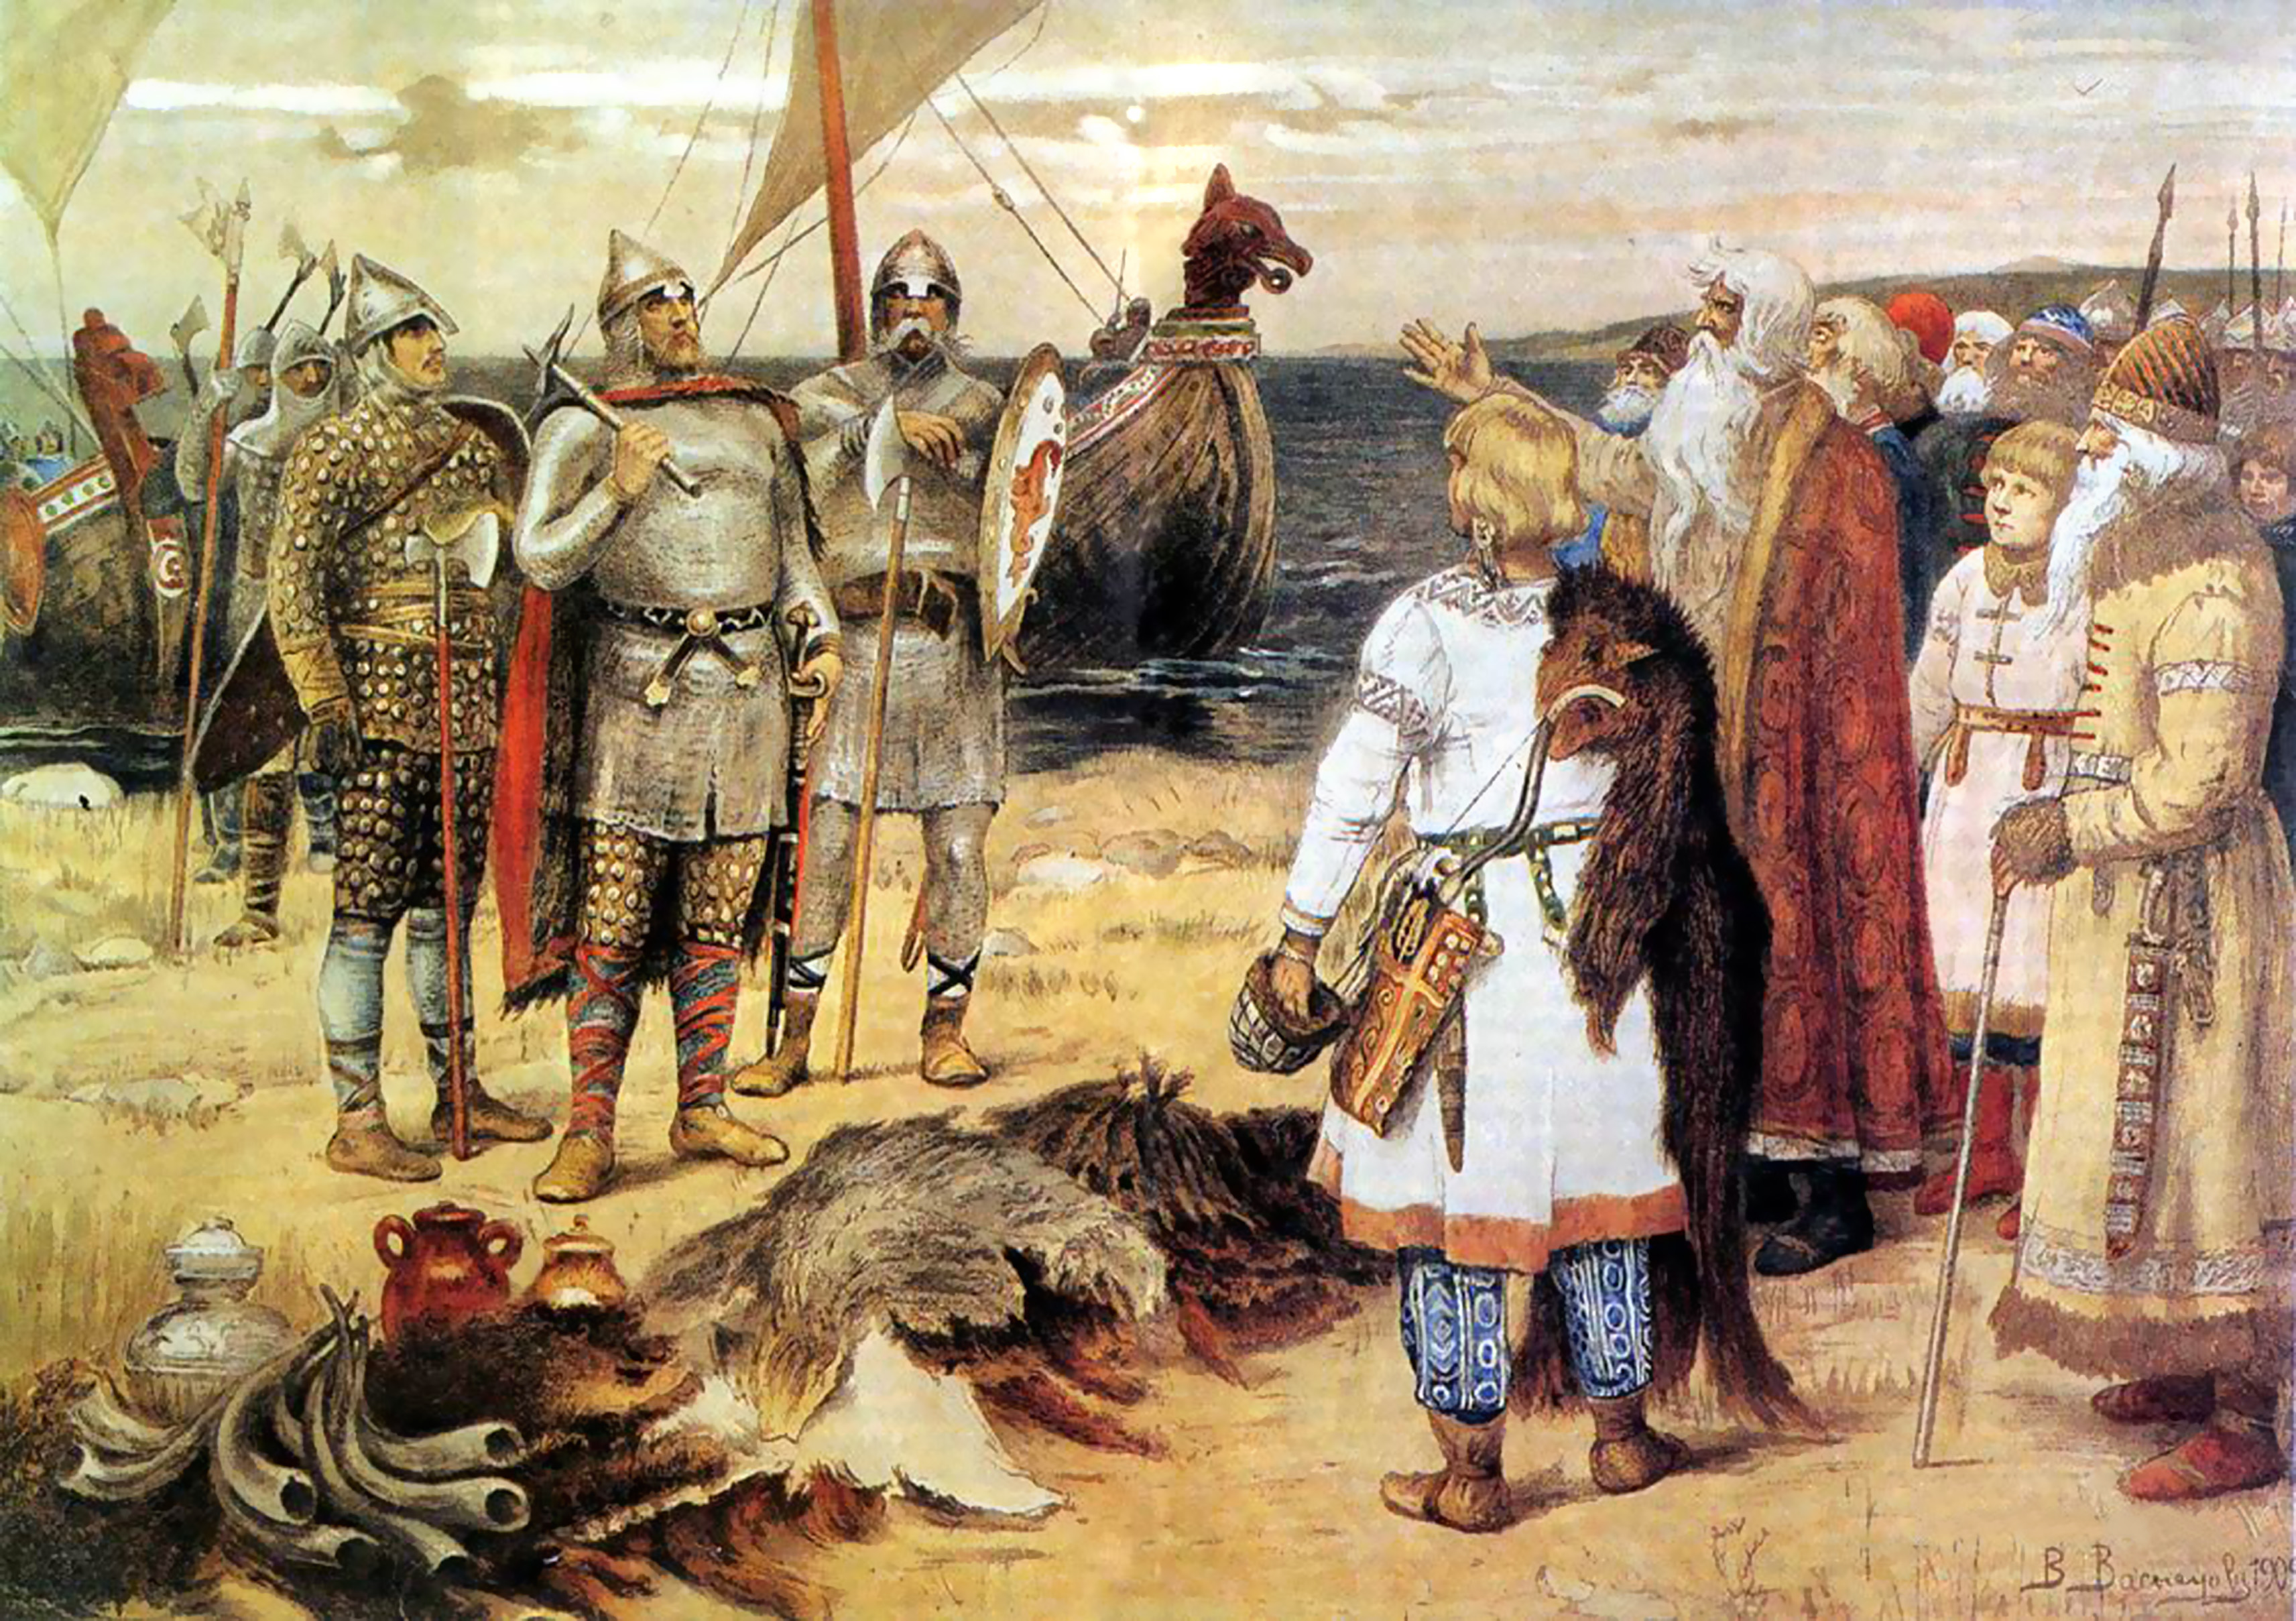
\includegraphics[width=0.45\textwidth]{img/rus/1.jpg}
    \caption{Призвание варягов}
    \label{fig:summon}
\end{figure}

\begin{figure}[ht]
    \centering
    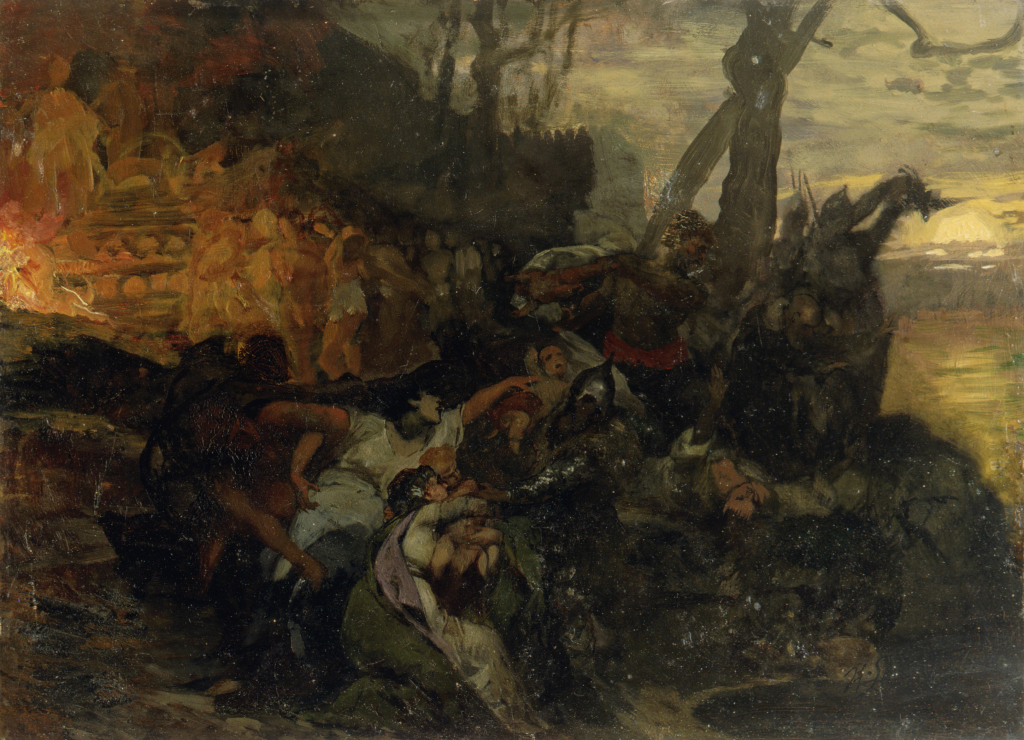
\includegraphics[width=0.45\textwidth]{img/rus/1afa34a7f984eeabdbb0a7d494132ee5_x1.png}
    \caption{Тризна дружинников Святослава после боя под Доростолом в 971 году}
    \label{fig:trizna}
\end{figure}

\begin{figure}[ht]
    \centering
    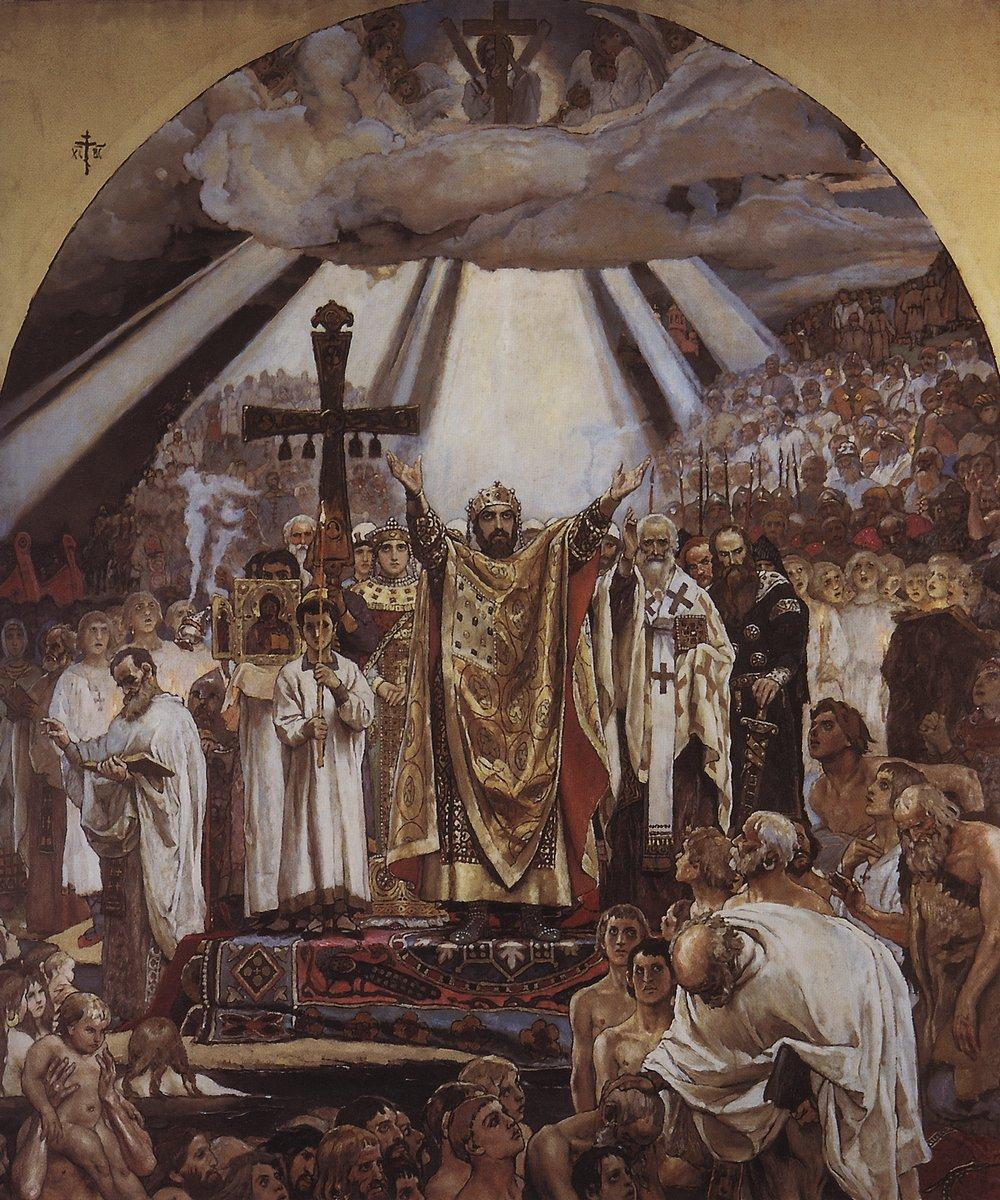
\includegraphics[width=0.45\textwidth]{img/rus/2.jpg}
    \caption{Крещение Руси}
    \label{fig:chresh}
\end{figure}

\begin{figure}[ht]
    \centering
    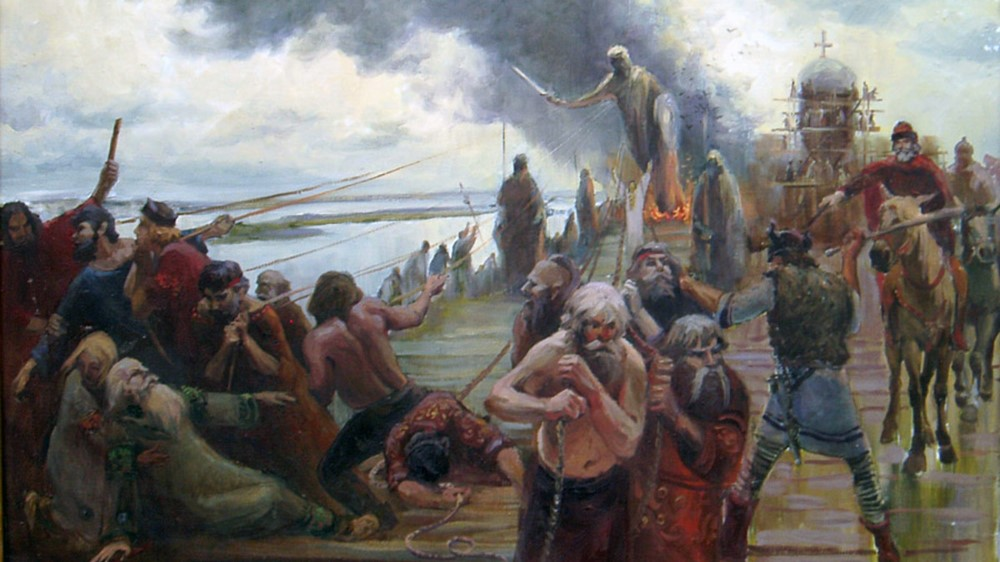
\includegraphics[width=0.45\textwidth]{img/rus/sverzh.jpg}
    \caption{Свержение идолов в Киеве}
    \label{fig:sverzh}
\end{figure}

\begin{figure}[ht]
    \centering
    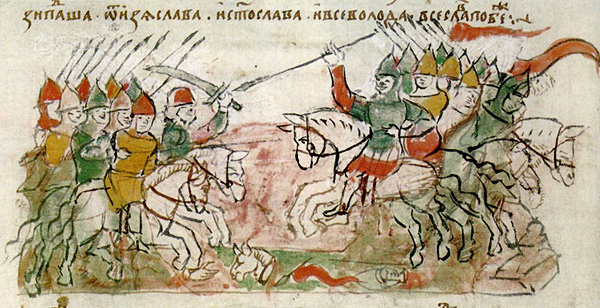
\includegraphics[width=0.45\textwidth]{img/rus/3.jpg}
    \caption{Битва на реке Немиге}
    \label{fig:nemiga}
\end{figure}

\begin{figure}[ht]
    \centering
    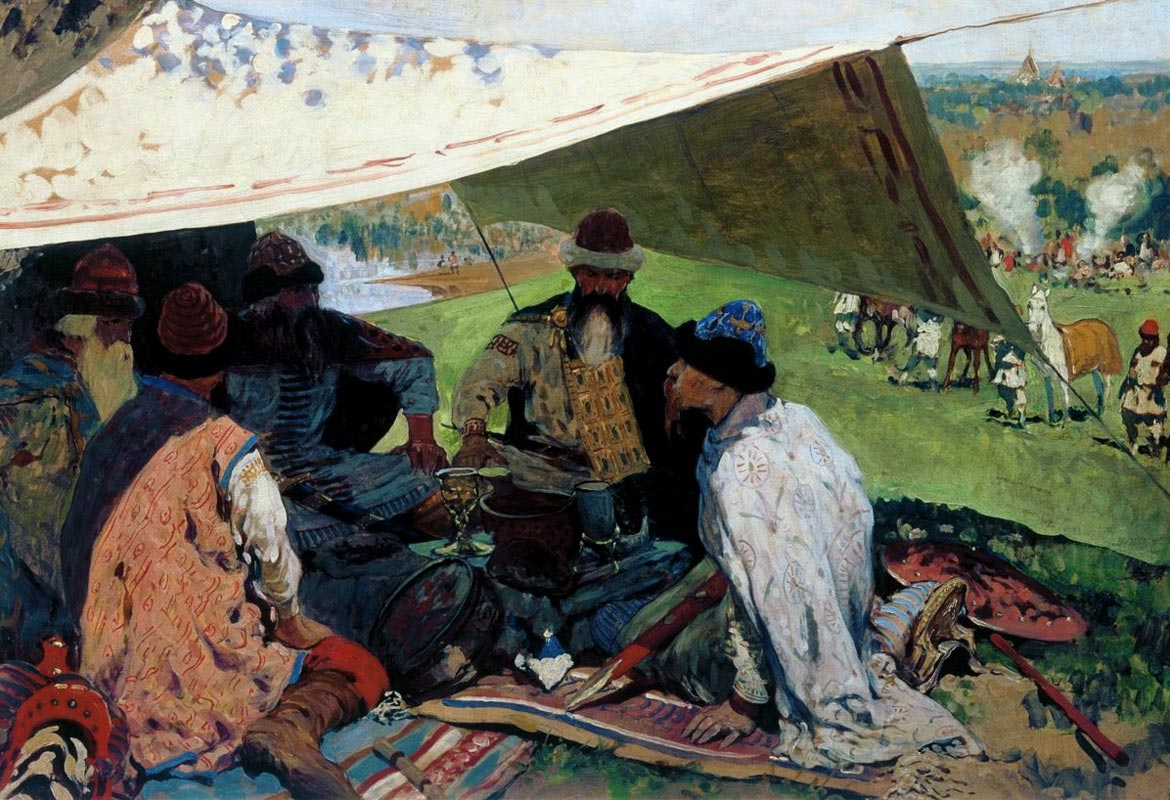
\includegraphics[width=0.45\textwidth]{img/rus/uvetichi.jpg}
    \caption{Русские князья заключают мир в Уветичах}
    \label{fig:uvetichi}
\end{figure}

\begin{figure}[ht]
    \centering
    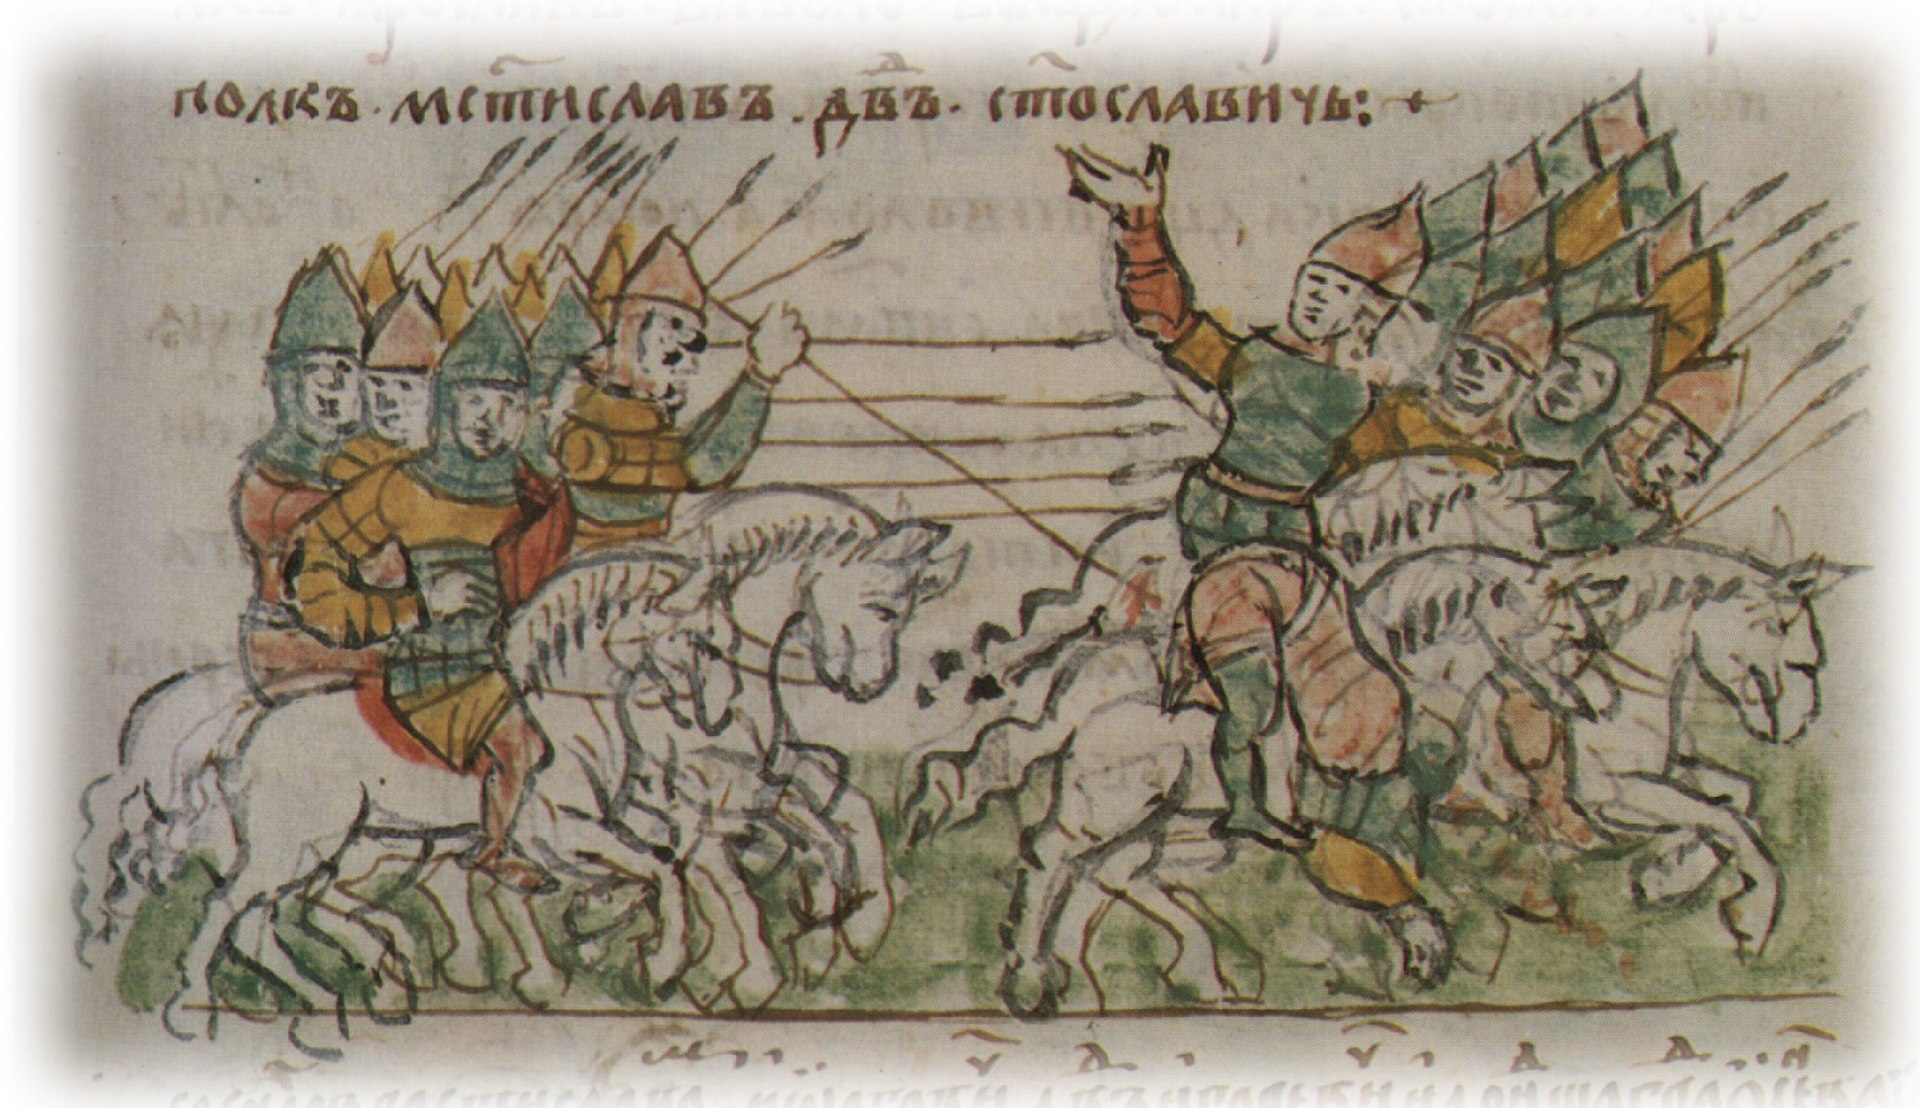
\includegraphics[width=0.45\textwidth]{img/rus/4.jpg}
    \caption{Битва при Салнице}
    \label{fig:salnitsa}
\end{figure}

\begin{figure}[ht]
    \centering
    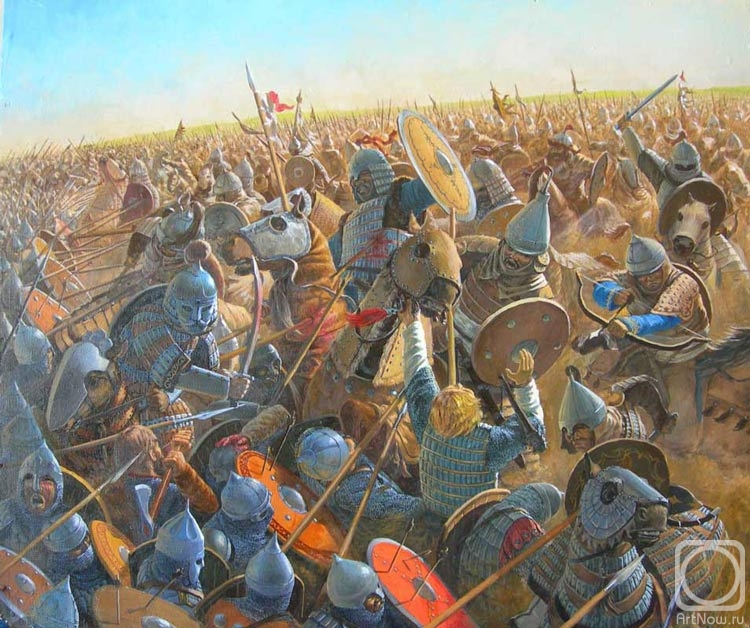
\includegraphics[width=0.45\textwidth]{img/rus/5.jpg}
    \caption{Битва при Калке}
    \label{fig:kalka}
\end{figure}


\begin{figure}[ht]
    \centering
    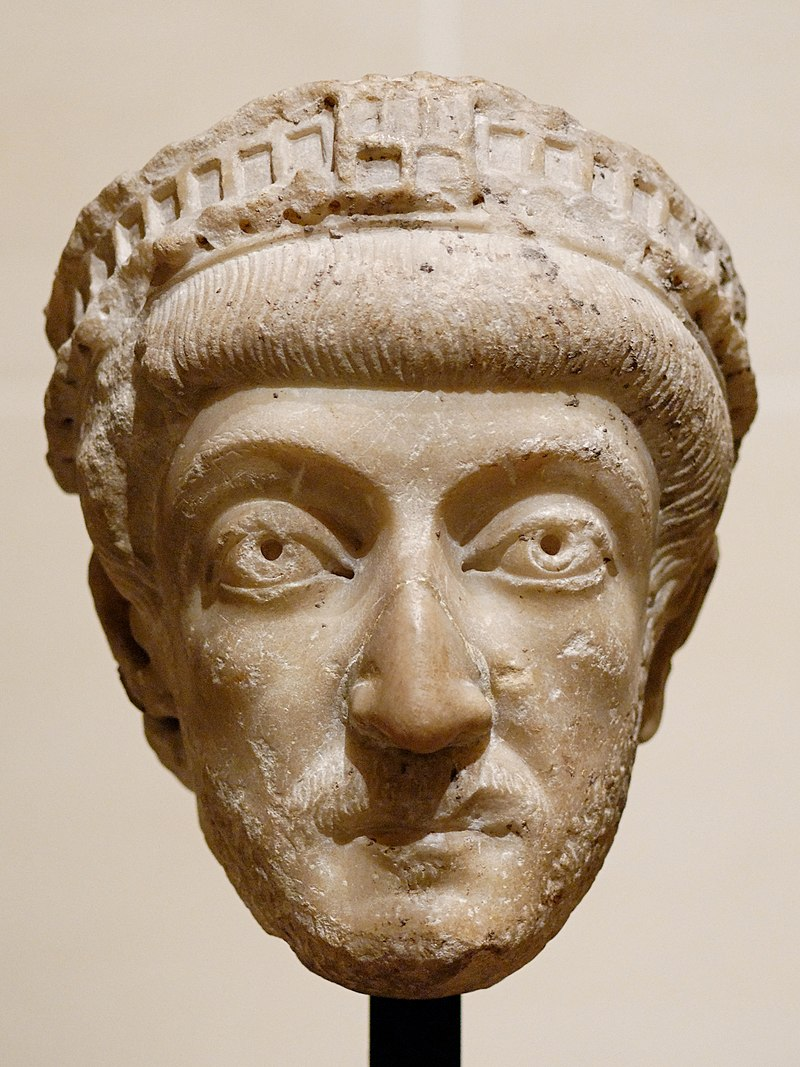
\includegraphics[width=0.45\textwidth]{img/vizant/1_800px-Theodosius_II_Louvre_Ma1036.jpg}
    \caption{Бюст Феодосия II}
    \label{fig:theodosius}
\end{figure}

\begin{figure}[ht]
    \centering
    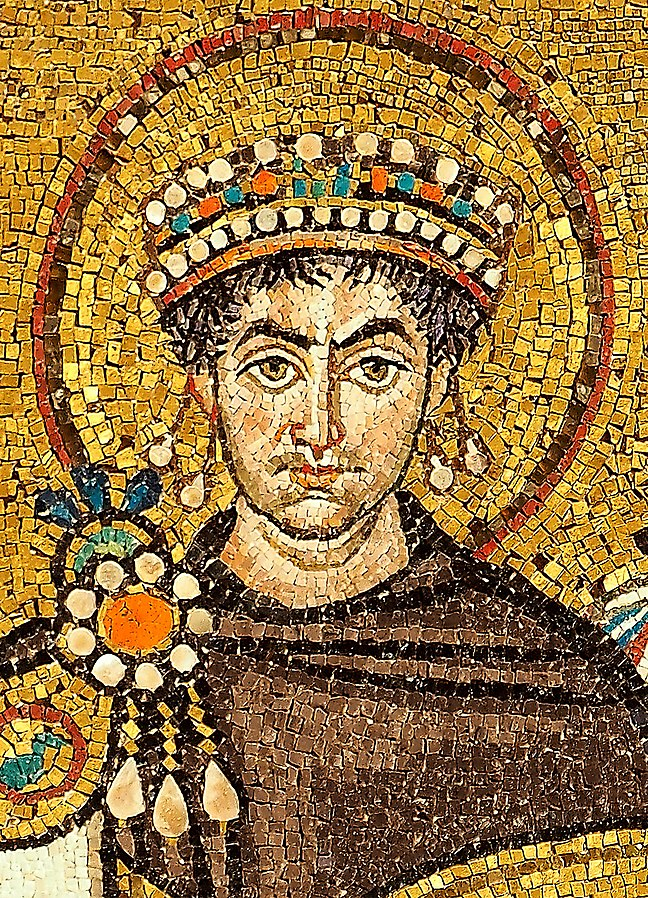
\includegraphics[width=0.45\textwidth]{img/vizant/2_Mosaic_of_Justinianus_I_-_Basilica_San_Vitale_(Ravenna).jpg}
    \caption{Бюст Феодосия II}
    \label{fig:justinianus}
\end{figure}

\begin{figure}[ht]
    \centering
    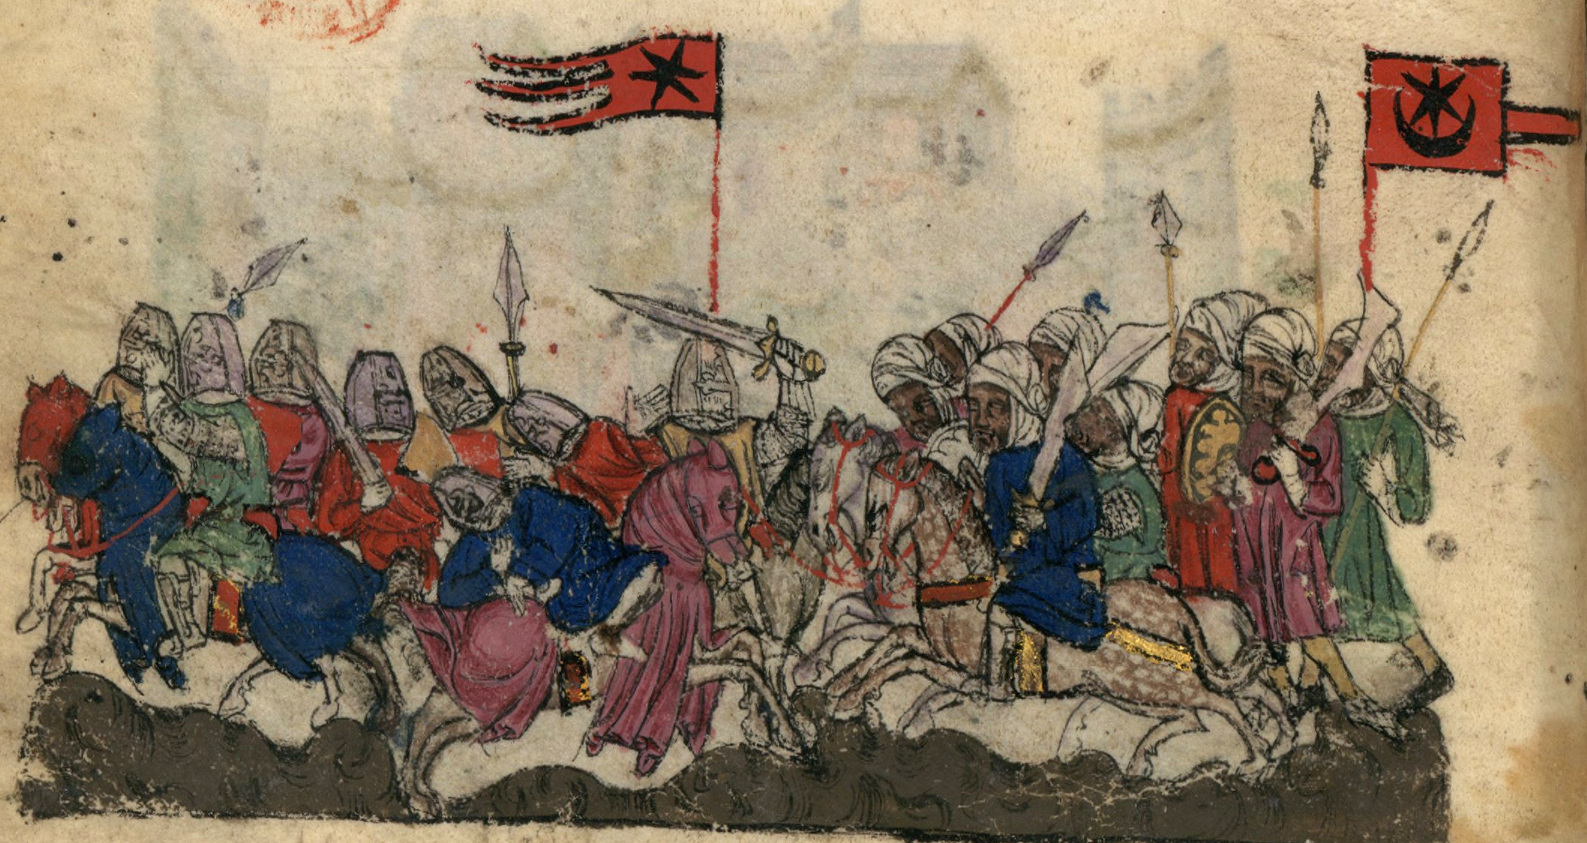
\includegraphics[width=0.45\textwidth]{img/vizant/3_Hayton_BNF886_9v.jpg}
    \caption{Битва при Ярмуке}
    \label{fig:yarmuka}
\end{figure}

\begin{figure}[ht]
    \centering
    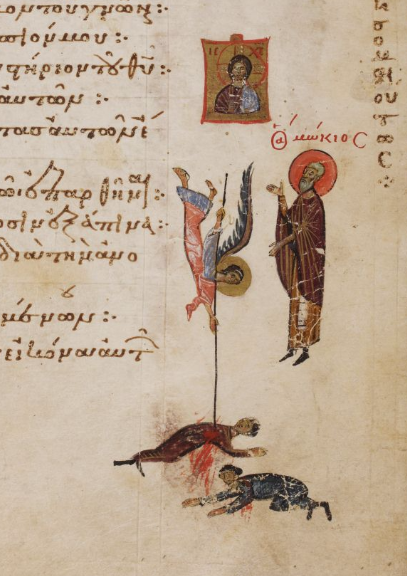
\includegraphics[width=0.45\textwidth]{img/vizant/4.jpg}
    \caption{Святой Мокий Амфипольский и ангел, убивающий иконоборцев}
    \label{fig:ikoni}
\end{figure}

\begin{figure}[ht]
    \centering
    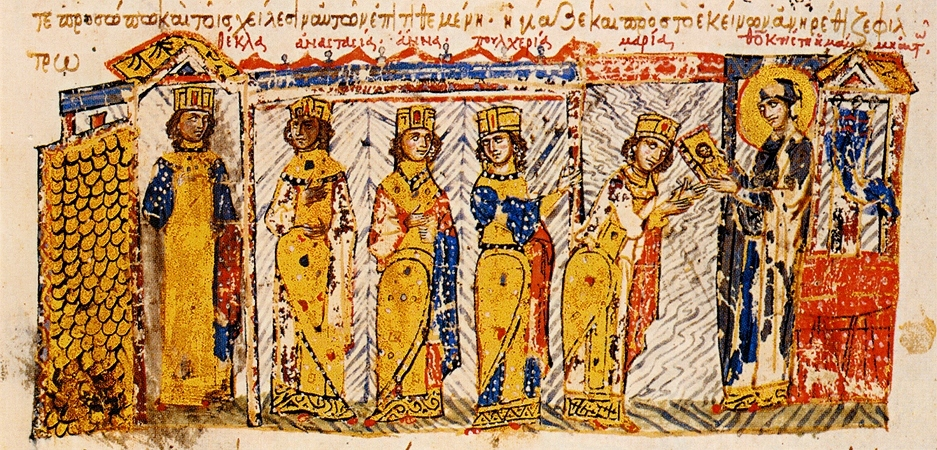
\includegraphics[width=0.45\textwidth]{img/vizant/5.jpg}
    \caption{Дочери императрицы Феодоры учатся почитать иконы у бабушки Феоктисты}
    \label{fig:feodora}
\end{figure}

\begin{figure}[ht]
    \centering
    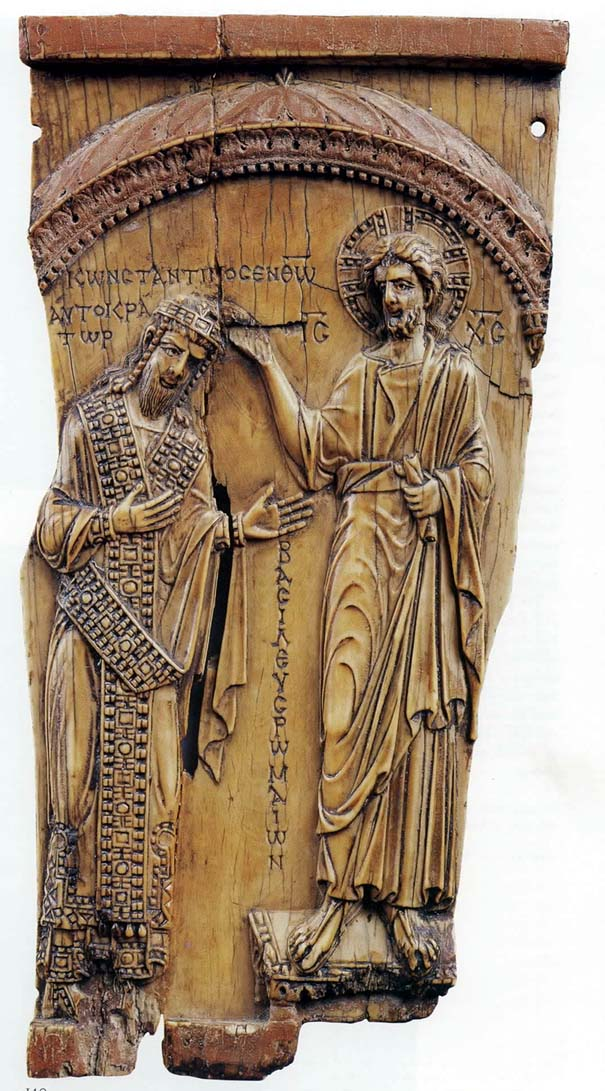
\includegraphics[width=0.45\textwidth]{img/vizant/6_Porphyrogenetus.jpg}
    \caption{Христос, благословляющий Константина Багрянородного}
    \label{fig:christ}
\end{figure}

\begin{figure}[ht]
    \centering
    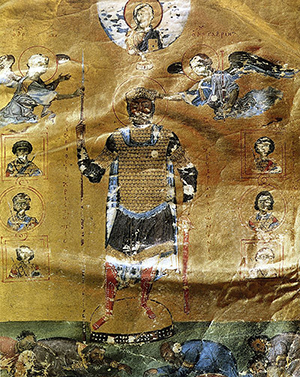
\includegraphics[width=0.45\textwidth]{img/vizant/7.jpg}
    \caption{Ангелы возлагают на Василия II императорскую корону}
    \label{fig:angels}
\end{figure}

\begin{figure}[ht]
    \centering
    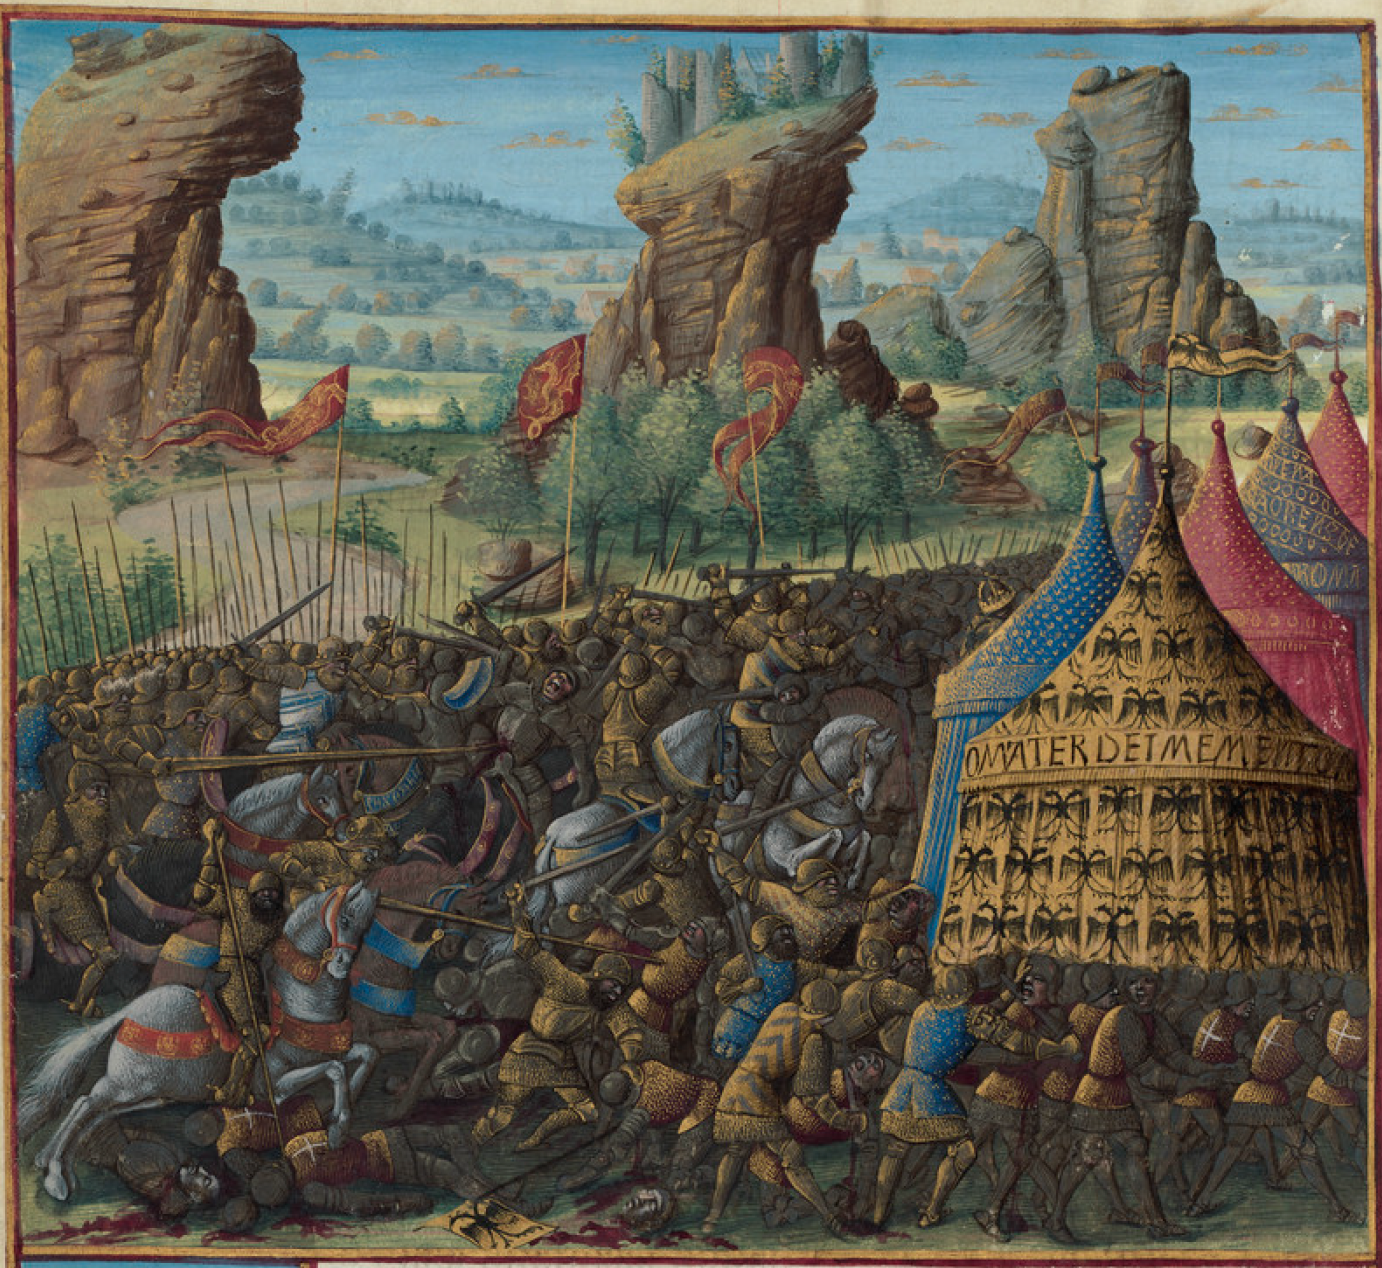
\includegraphics[width=0.45\textwidth]{img/vizant/Passages_faiz_oultre_mer_SEBASTIEN_MAMEROT_140_(cropped).png}
    \caption{Битва при Дорилее}
    \label{fig:dorilee}
\end{figure}


\begin{figure}[ht]
    \centering
    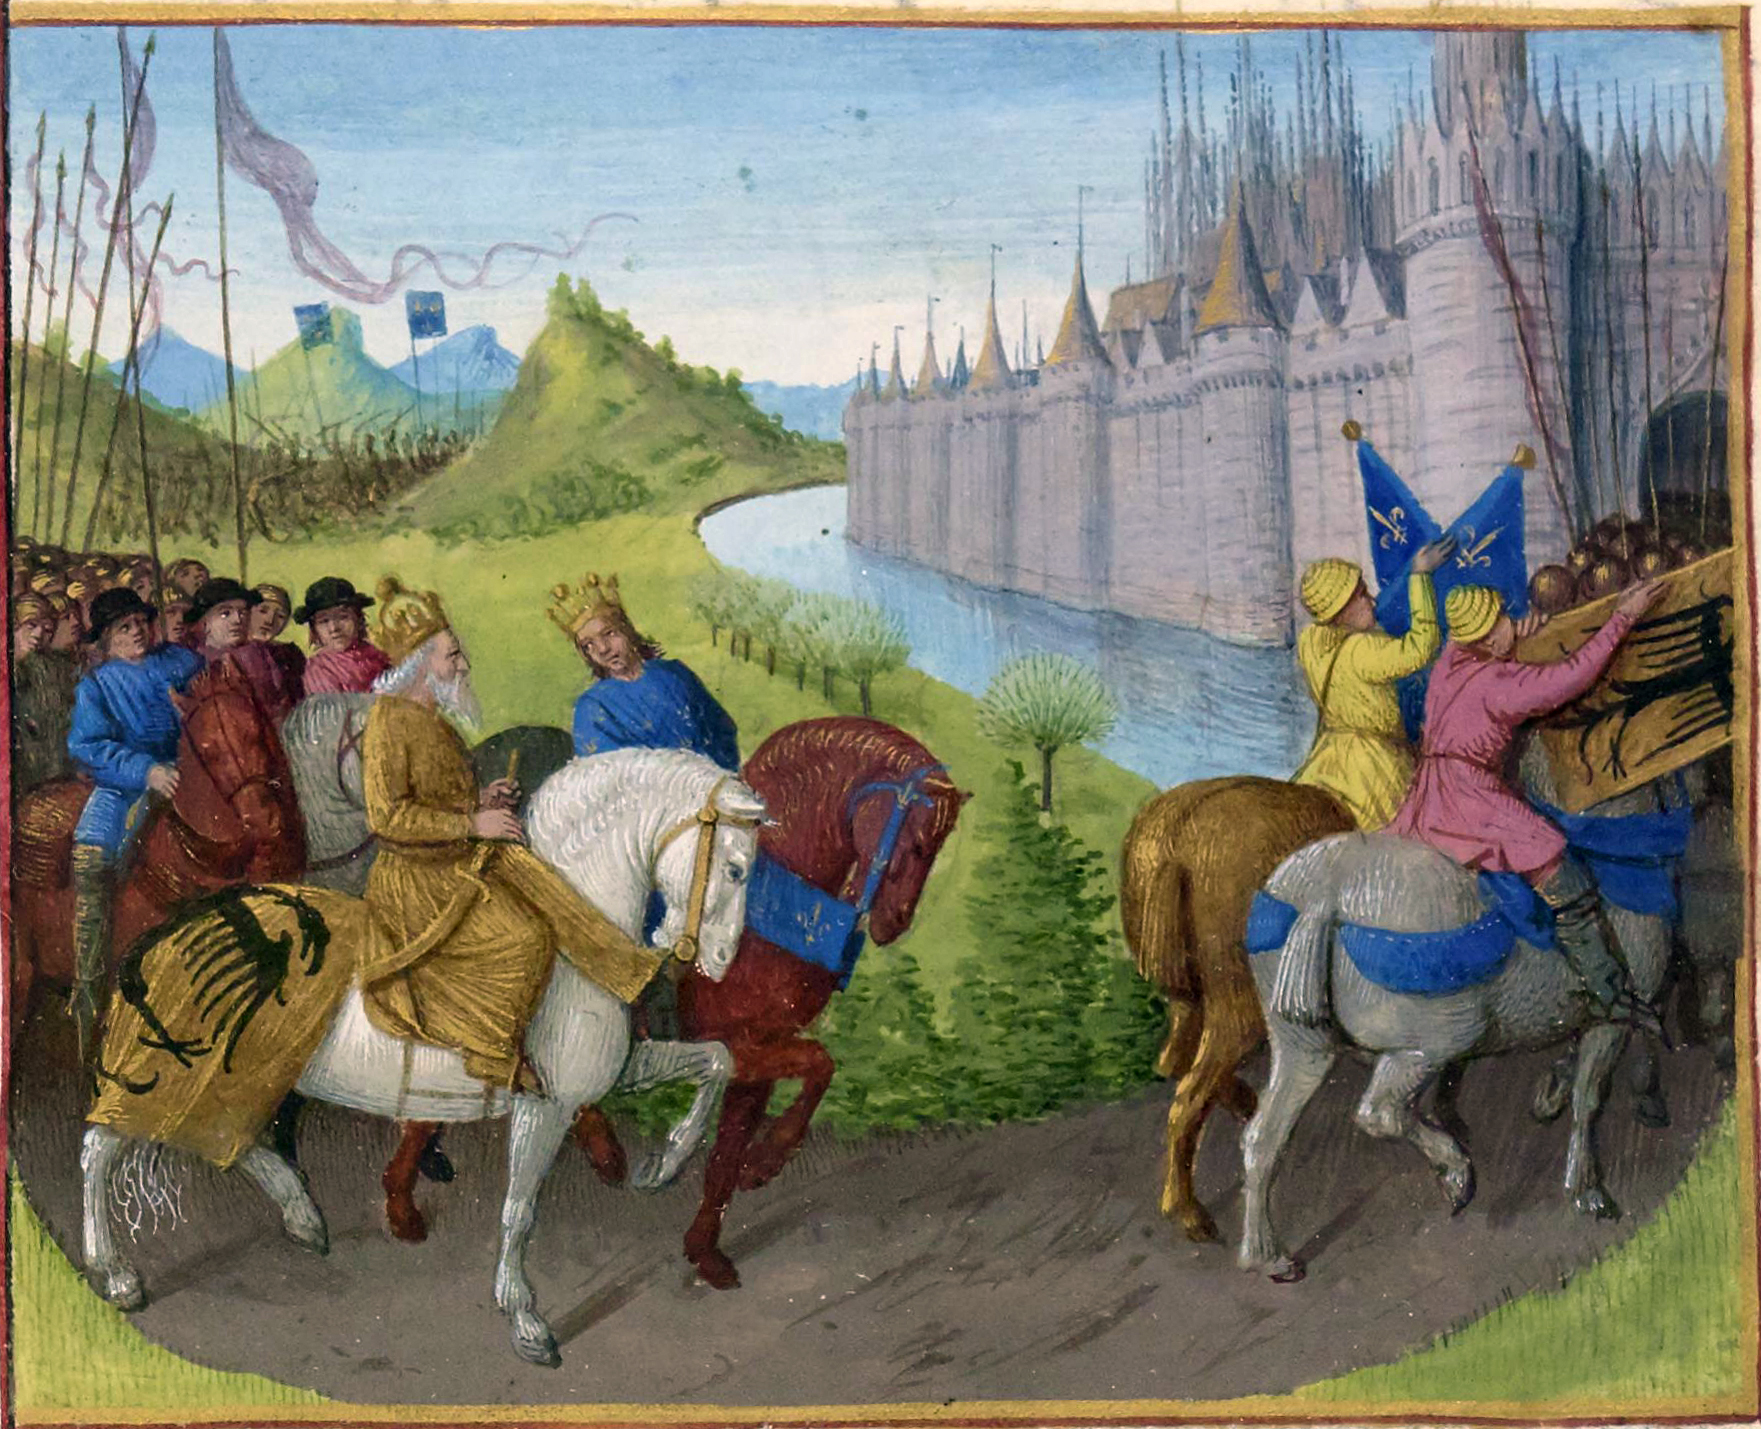
\includegraphics[width=0.45\textwidth]{img/vizant/8.jpg}
    \caption{Участники Второго крестового похода (1145—1149) прибывают в Константинополь}
    \label{fig:crusaders_2}
\end{figure}

\begin{figure}[ht]
    \centering
    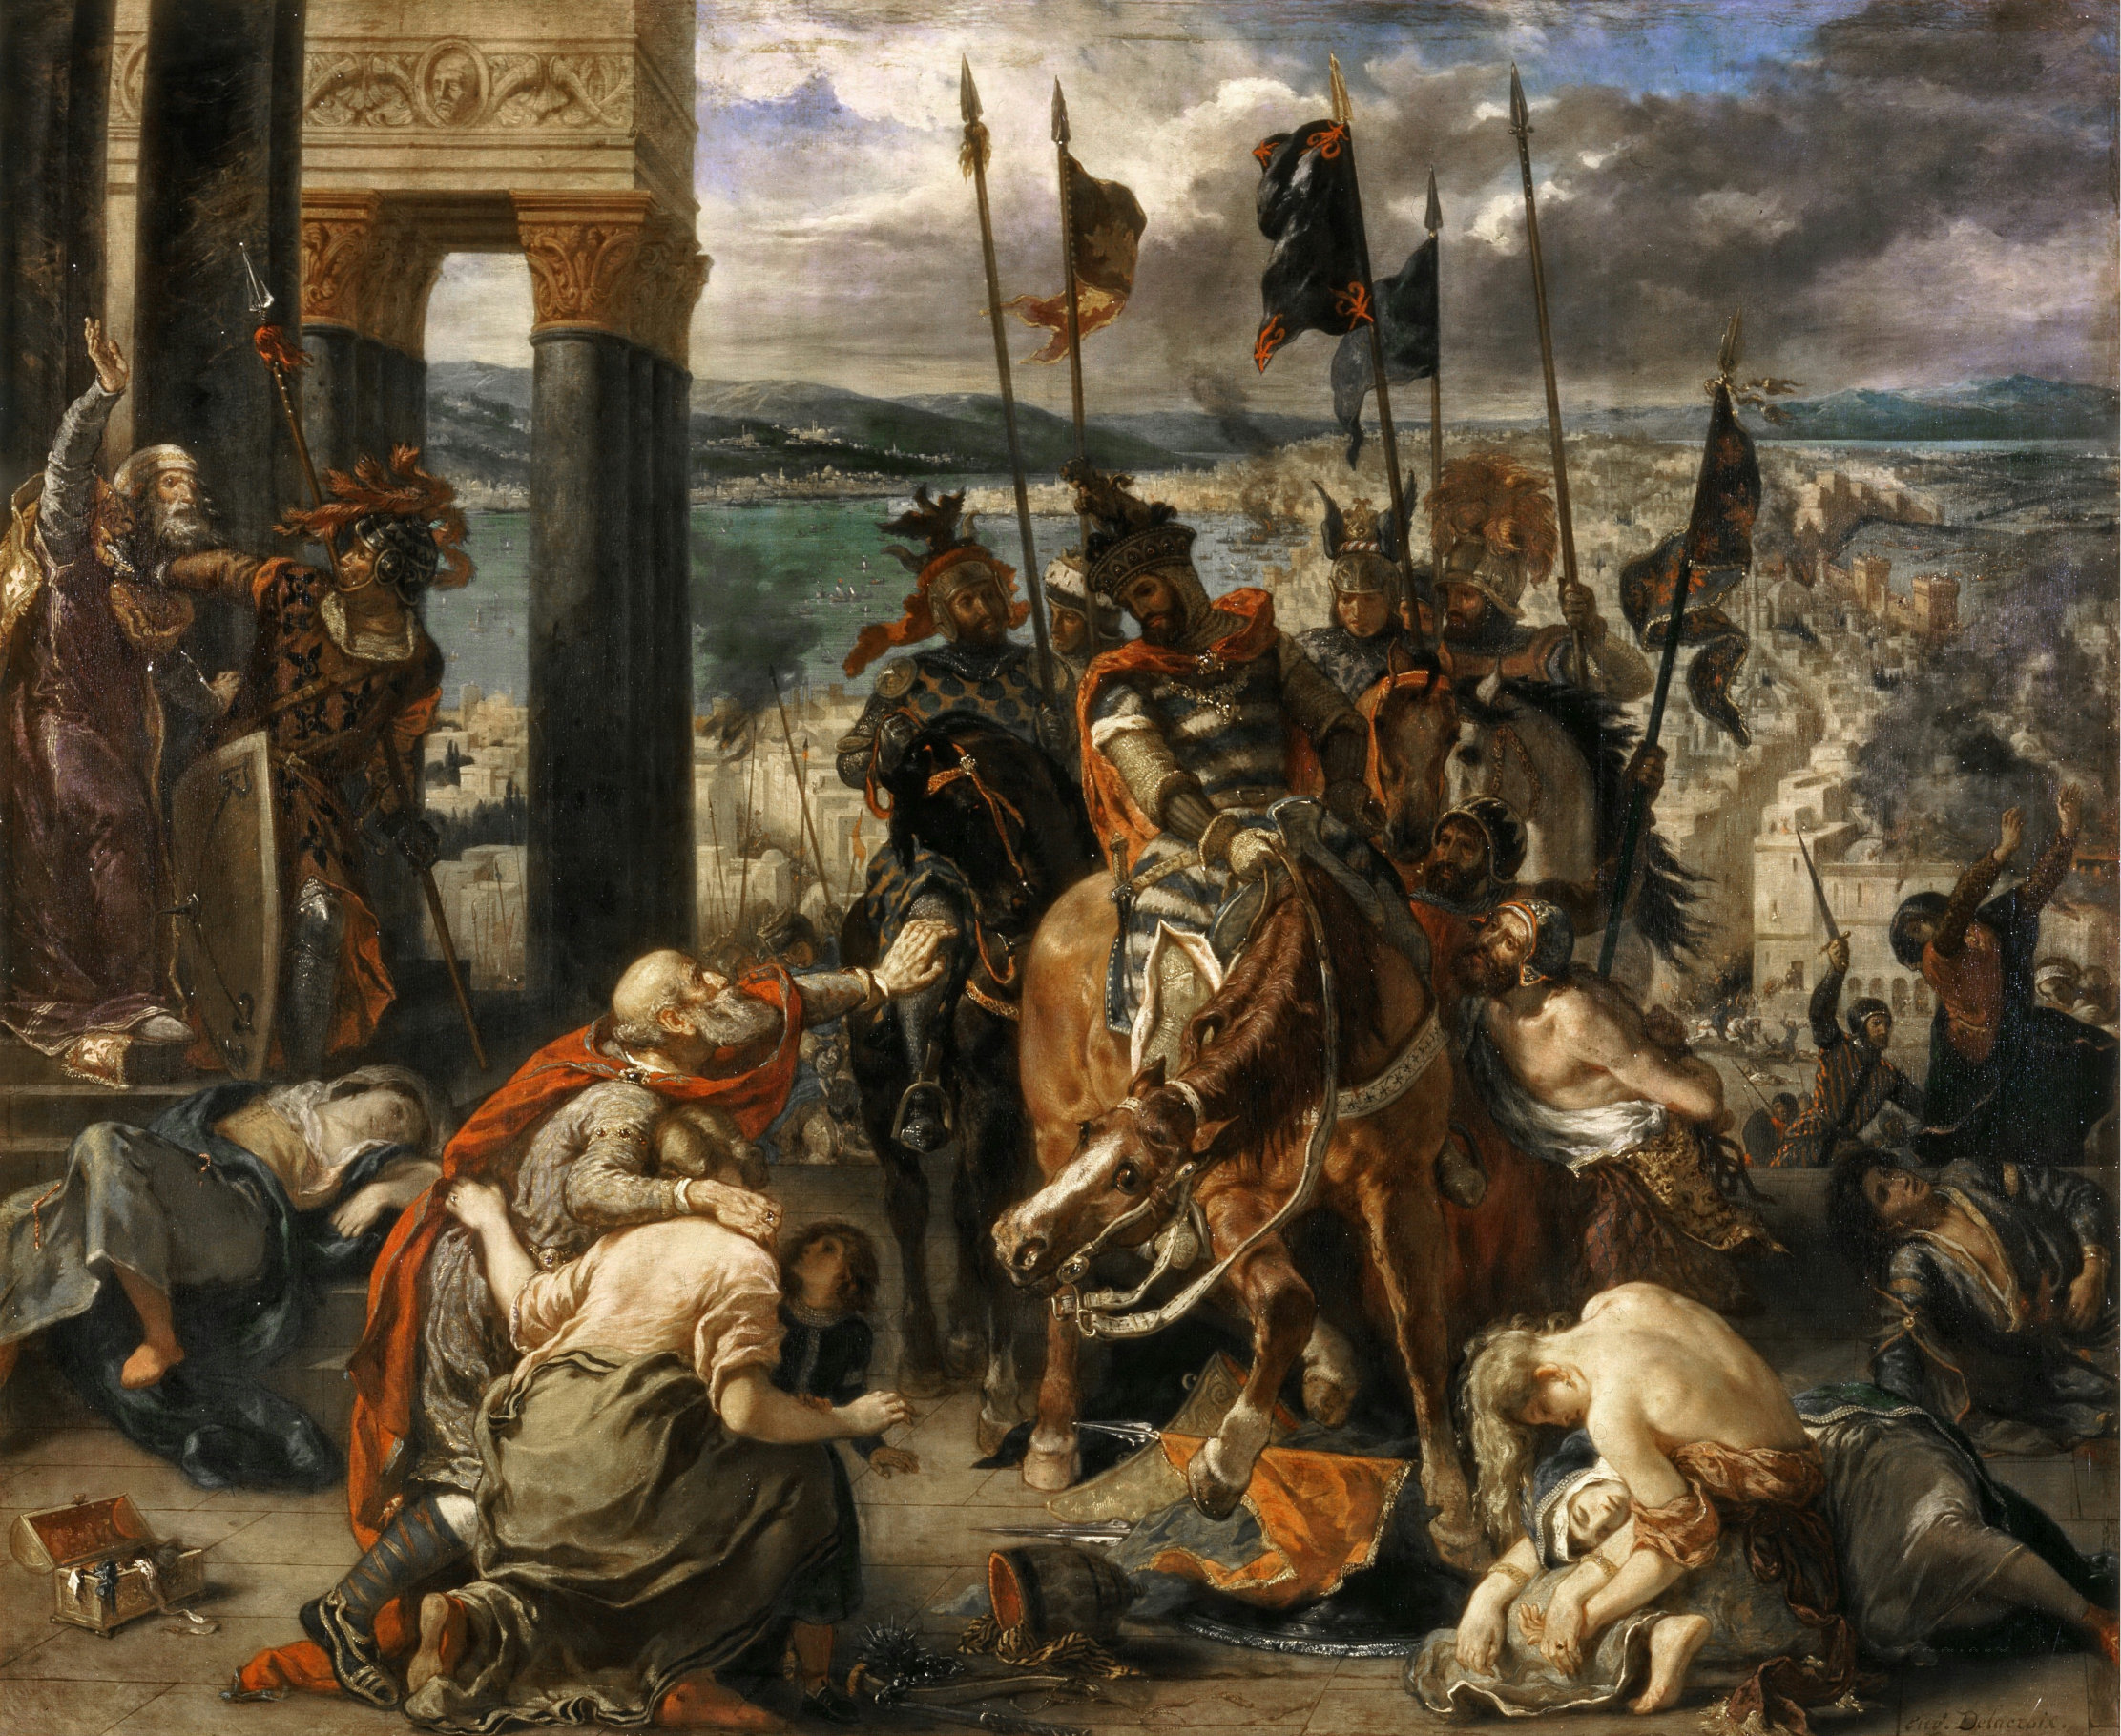
\includegraphics[width=0.45\textwidth]{img/vizant/9.jpg}
    \caption{Взятие Константинополя крестоносцами (1204 г.)}
    \label{fig:crusaders_3}
\end{figure}

\begin{figure}[ht]
    \centering
    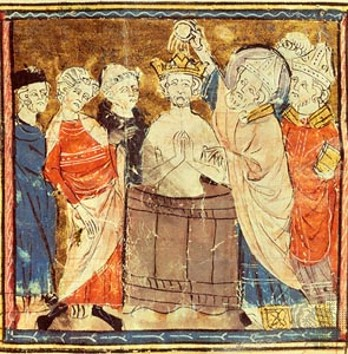
\includegraphics[width=0.45\textwidth]{img/europe/clovis.jpg}
    \caption{Крещение Хлодвига}
    \label{fig:clovis}
\end{figure}

\begin{figure}[ht]
    \centering
    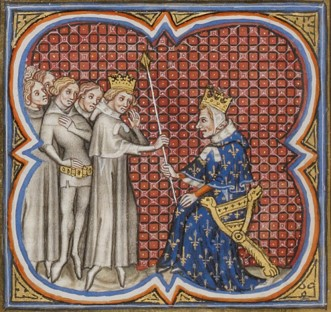
\includegraphics[width=0.45\textwidth]{img/europe/gunt.jpg}
    \caption{Гунтрамн и Хильдеберт}
    \label{fig:gunt}
\end{figure}

\begin{figure}[ht]
    \centering
    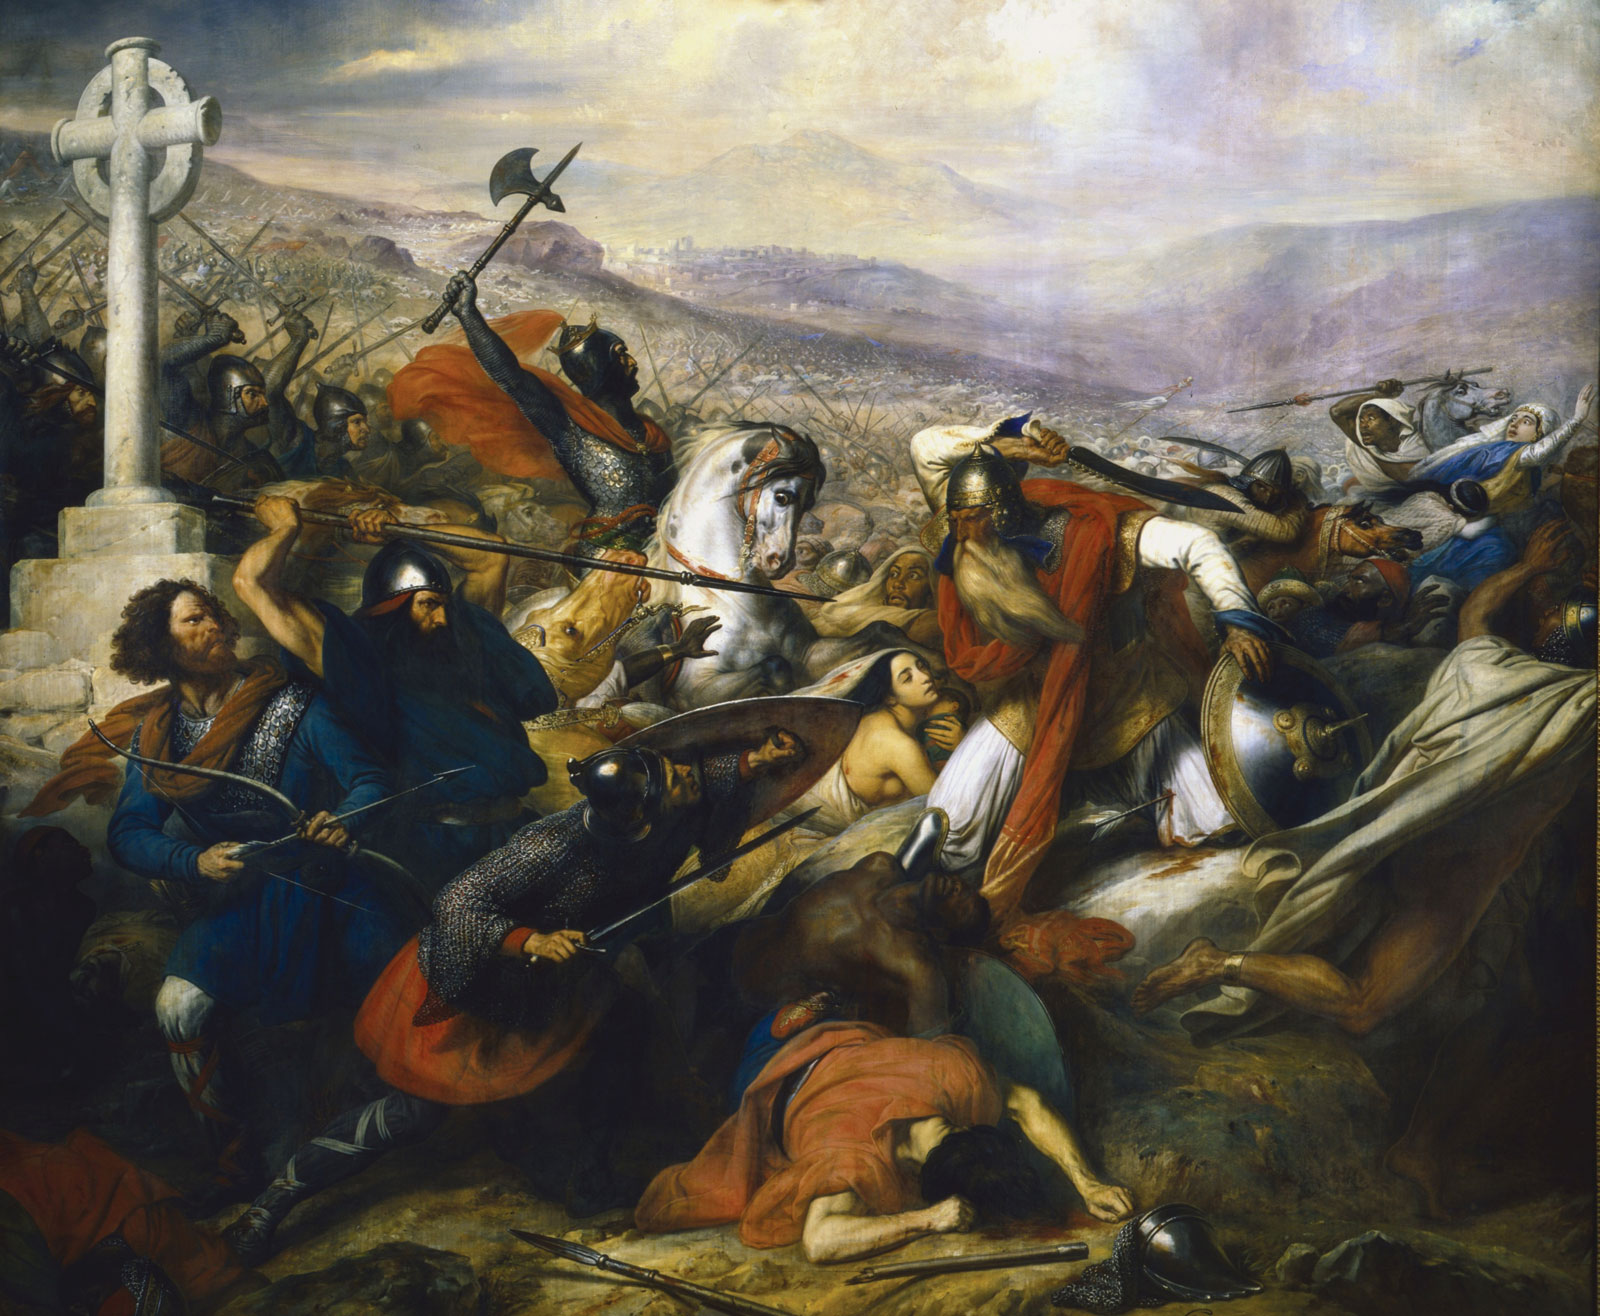
\includegraphics[width=0.45\textwidth]{img/europe/poitiers.png}
    \caption{Битва при Пуатье (732 г.)}
    \label{fig:poitiers}
\end{figure}

\begin{figure}[ht]
    \centering
    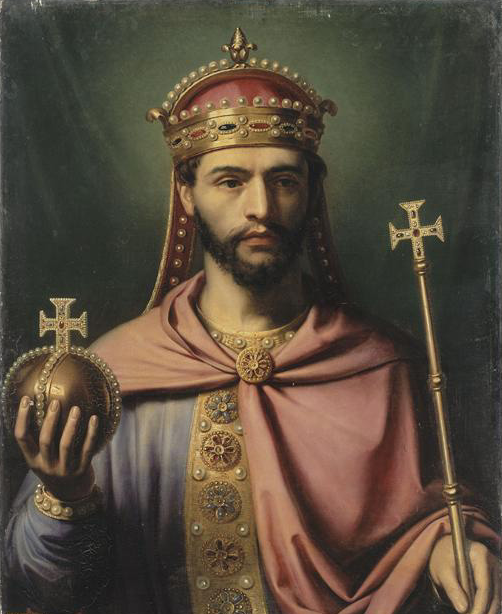
\includegraphics[width=0.45\textwidth]{img/europe/Louis_le_Pieux.png}
    \caption{Людовик I Благочестивый, император Запада}
    \label{fig:louis}
\end{figure}

\begin{figure}[ht]
    \centering
    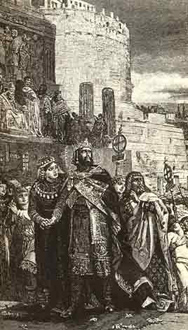
\includegraphics{img/europe/Marozia_bertolini.jpg}
    \caption{Свадьба Гуго и Мароции}
    \label{fig:gugo}
\end{figure}

\begin{figure}[ht]
    \centering
    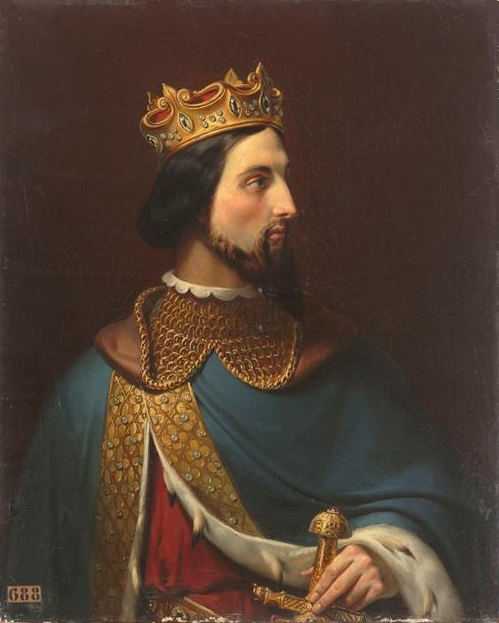
\includegraphics[width=0.45\textwidth]{img/europe/Blondel_-_Henry_I_of_France.jpg}
    \caption{Генрих I. Король Франции}
    \label{fig:henry}
\end{figure}

\begin{figure}[ht]
    \centering
    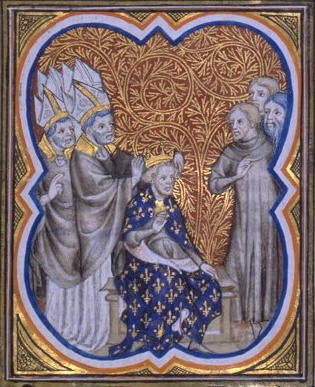
\includegraphics[width=0.45\textwidth]{img/europe/LudvikVIFrr.jpg}
    \caption{Коронация Людовика VI}
    \label{fig:corona}
\end{figure}

\begin{figure}[ht]
    \centering
    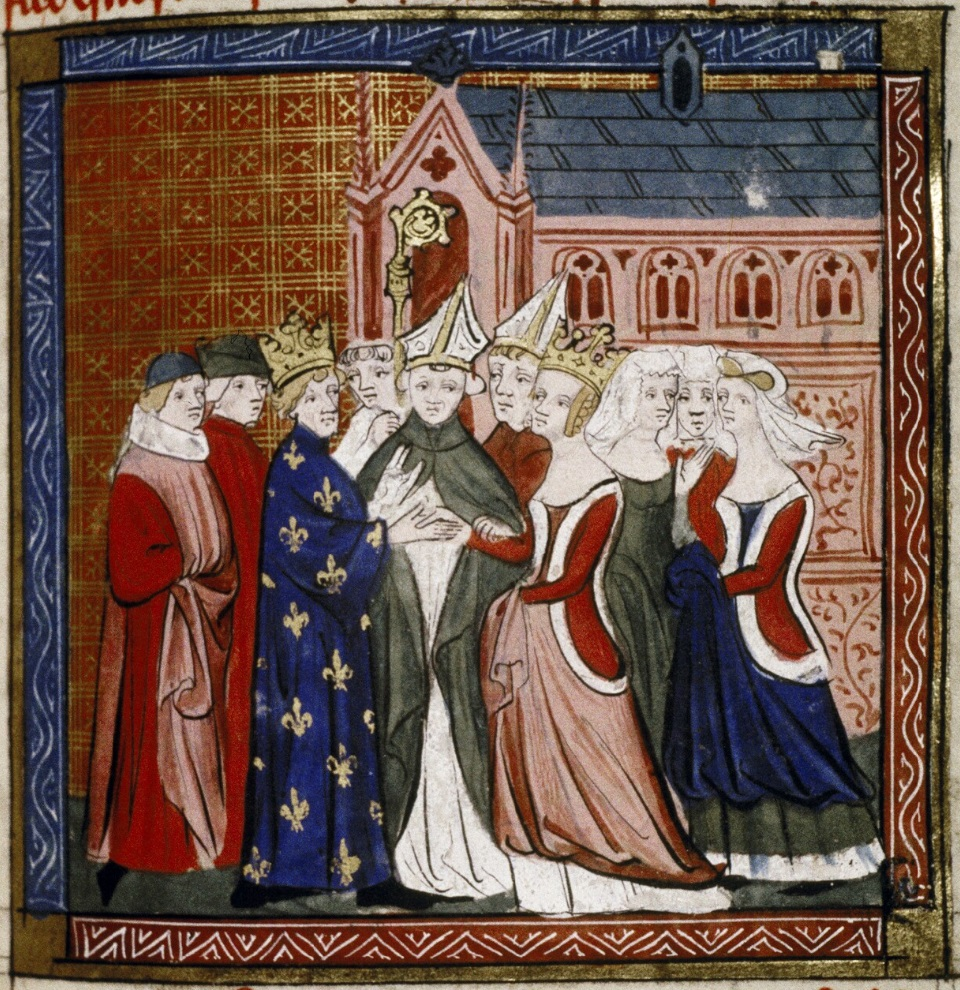
\includegraphics[width=0.45\textwidth]{img/europe/aleonora.jpg}
    \caption{Свадьба Алиеноры Аквитанской и Людовика VII}
    \label{fig:marriage}
\end{figure}

\begin{figure}[ht]
    \centering
    \includegraphics[width=0.45\textwidth]{img/europe/Français_5594,_fol._205_haut,_Bataille_de_Tyr_(1187).jpeg}
    \caption{Осада Тира (1187)}
    \label{fig:tyr}
\end{figure}

\begin{figure}[ht]
    \centering
    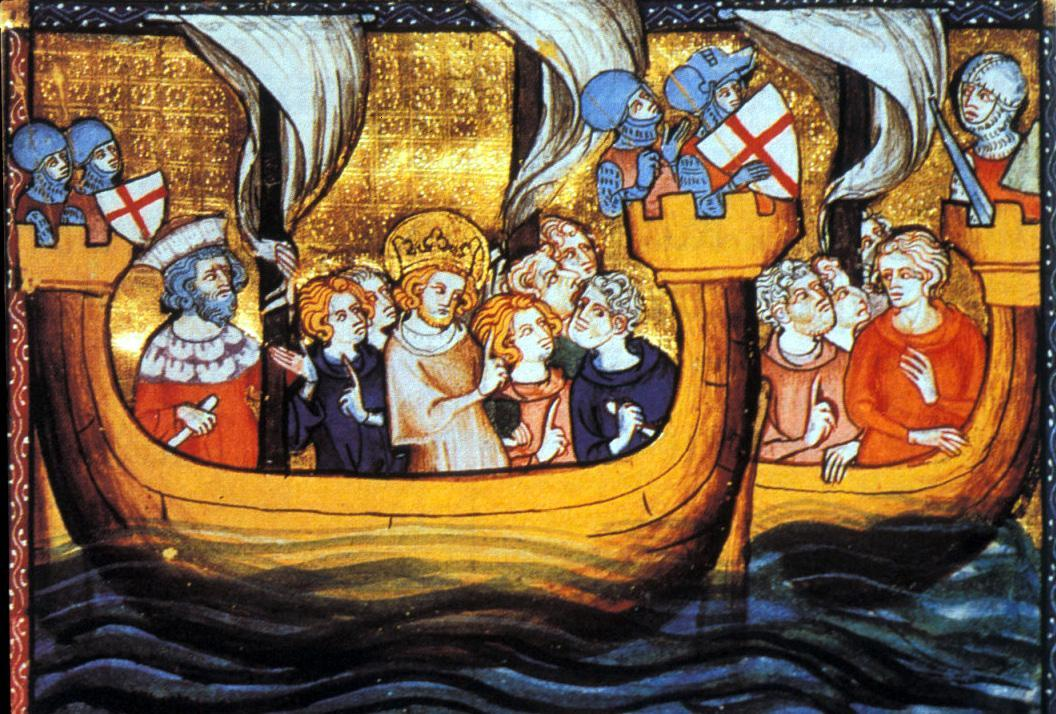
\includegraphics[width=0.45\textwidth]{img/europe/Seventh_crusade.jpg}
    \caption{Людовик IX с войсками в Крестовом походе}
    \label{fig:crusaders}
\end{figure}


\end{document}